\section{Introdução ao controle de processos industriais}

\begin{frame}{Introdução}
	\begin{block}{O que é a teoria de controle?}
		\begin{itemize}
			\item Trata-se do estudo de \textbf{como} levar um processo a um ponto de equilíbrio, ou seja, à \textbf{estabilidade}.
			\item Seja no piloto automático de um avião, ou na indústria, a \textbf{teoria de controle} é usada.
		\end{itemize}
	\end{block}

	\begin{minipage}{0.49\linewidth}
		\centering
		\includegraphics[width=1\linewidth]{Figuras/Ch11/fig1}
	\end{minipage}
	\hfill
	\begin{minipage}{0.49\linewidth}
		\centering
		\includegraphics[width=1\linewidth]{Figuras/Ch11/fig2}
	\end{minipage}
\end{frame}


\begin{frame}{Estabilidade}
	\begin{block}{O que é estabilidade?}
		\begin{itemize}
			\item A estabilidade é a medida da facilidade que um processo tem de retornar a um ponto de equilíbrio.
		\end{itemize}
	\end{block}

	\vspace{0.5cm}
	
	\begin{minipage}{0.49\linewidth}
		\centering
		\scalebox{1}{\begin{tikzpicture}[scale=0.5]
			\draw (-4,-3) rectangle (4,3); %CLP
		\draw (-4,0) -- (-2.5,0); %Div in out
		\draw (-2.5,-3) -- (-2.5,3); %Div cartoes
		\draw (-1.5,-2.5) rectangle (0,2.5); %Mem dados
		\draw (0.5,-2.5) rectangle (3.5,-1); %Mem prog
		\draw (1,0) rectangle (3,2); %CPU
		\draw (-4,-5) rectangle (4,-3); %Alimentacao
		\draw (-2.5,4) rectangle (4,6); %Term de prog
		
		\draw (1,2.6) node {CLP};
		
		\draw (-3.25,1.5) node[text width=1.5cm,align=center,rotate=90] {\small Cartões de input};
		
		\draw (-3.25,-1.5) node[text width=1.5cm,align=center,rotate=90] {\small Cartões de output};
		
		\node at (2,1) {\small CPU};
		
		\node[rotate=90,text width=1.5cm,align=center] at (-0.75,0) {\small Memória de dados};
		
		\node[text width=2cm,align=center] at (2,-1.75) {\footnotesize Memória de programa};
		
		\node at (-6,0) {Campo};
		
		\node at (0,-4) {Alimentação};
		
		\node[text width=3cm,align=center] at (0.75,5) {Terminal de programação};
		
		\draw[-Latex] (-8,1.5) -- node[above] {Entradas} +(4,0);
		\draw[Latex-] (-8,-1.5) -- node[below] {Saídas} +(4,0);
		\draw[-Latex] (-2.5,1.5) -- +(1,0);
		\draw[Latex-] (-2.5,-1.5) -- +(1,0);
		\draw[-Latex] (0,1.5) -- +(1,0);
		\draw[Latex-] (0,0.5) -- +(1,0);
		\draw[Latex-] (2,0) -- +(0,-1);
		
		\draw[-Latex] (-1.5,4) -- +(0,-1);
		\draw[Latex-] (3,4) -- +(0,-1);
	\end{tikzpicture}}
	\end{minipage}
	\hfill
	\begin{minipage}{0.49\linewidth}
		\centering
		\scalebox{1}{

\tikzset{every picture/.style={line width=0.75pt}} %set default line width to 0.75pt        

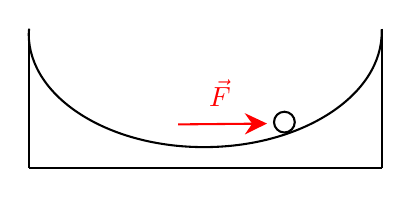
\begin{tikzpicture}[x=0.75pt,y=0.75pt,yscale=-1,xscale=1]
%uncomment if require: \path (0,300); %set diagram left start at 0, and has height of 300

%Straight Lines [id:da3398984480833569] 
\draw    (90,103) -- (90,170) ;


%Straight Lines [id:da39213437306955434] 
\draw    (260,103) -- (260,170) ;


%Straight Lines [id:da7536538469625644] 
\draw    (90,170) -- (260,170) ;


%Shape: Arc [id:dp6883804097522237] 
\draw  [draw opacity=0] (260,103) .. controls (260,103) and (259.87,104.01) .. (259.88,104.37) .. controls (260.12,134.75) and (222.24,159.67) .. (175.28,160.04) .. controls (128.31,160.41) and (90.05,136.08) .. (89.81,105.71) .. controls (89.81,105.53) and (89.81,105.35) .. (89.81,105.17) -- (174.84,105.04) -- cycle ; \draw   (259.85,103.29) .. controls (259.87,103.65) and (259.87,104.01) .. (259.88,104.37) .. controls (260.12,134.75) and (222.24,159.67) .. (175.28,160.04) .. controls (128.31,160.41) and (90.05,136.08) .. (89.81,105.71) .. controls (89.81,105.53) and (90,103) .. (90,103) ;
%Shape: Circle [id:dp54266808828771] 
\draw   (208,148) .. controls (208,145.24) and (210.24,143) .. (213,143) .. controls (215.76,143) and (218,145.24) .. (218,148) .. controls (218,150.76) and (215.76,153) .. (213,153) .. controls (210.24,153) and (208,150.76) .. (208,148) -- cycle ;
%Straight Lines [id:da8066991195909812] 
\draw [color={rgb, 255:red, 255; green, 0; blue, 0 }  ,draw opacity=1 ]   (161.8,149.1) -- (202.6,148.72) ;
\draw [shift={(204.6,148.7)}, rotate = 539.46] [fill={rgb, 255:red, 255; green, 0; blue, 0 }  ,fill opacity=1 ][line width=0.75]  [draw opacity=0] (10.72,-5.15) -- (0,0) -- (10.72,5.15) -- (7.12,0) -- cycle    ;


% Text Node
\draw (120,147) node  [align=left] {};
% Text Node
\draw (182,133.8) node [color={rgb, 255:red, 255; green, 0; blue, 0 }  ,opacity=1 ]  {$\vec{F}$};


\end{tikzpicture}
}
	\end{minipage}

	\vspace{0.5cm}

	\centering
	
	\Large	
	Sistema estável
\end{frame}


\begin{frame}{Estabilidade}
	\begin{minipage}{0.49\linewidth}
		\centering
		\scalebox{1}{

\tikzset{every picture/.style={line width=0.75pt}} %set default line width to 0.75pt        

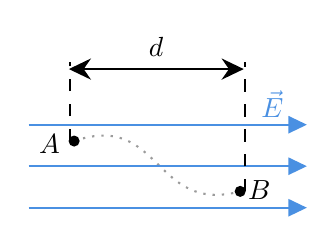
\begin{tikzpicture}[x=0.75pt,y=0.75pt,yscale=-1,xscale=1]
%uncomment if require: \path (0,300); %set diagram left start at 0, and has height of 300

%Curve Lines [id:da6177490068384819] 
\draw [color={rgb, 255:red, 155; green, 155; blue, 155 }  ,draw opacity=1 ] [dash pattern={on 0.84pt off 2.51pt}]  (137.88,127.88) .. controls (180,113.4) and (176,163.4) .. (217.88,152.13) ;


%Straight Lines [id:da7124330895115376] 
\draw [color={rgb, 255:red, 74; green, 144; blue, 226 }  ,draw opacity=1 ]   (116,120) -- (247,120) ;
\draw [shift={(250,120)}, rotate = 180] [fill={rgb, 255:red, 74; green, 144; blue, 226 }  ,fill opacity=1 ][line width=0.08]  [draw opacity=0] (8.93,-4.29) -- (0,0) -- (8.93,4.29) -- cycle    ;

%Straight Lines [id:da12792354611605283] 
\draw [color={rgb, 255:red, 74; green, 144; blue, 226 }  ,draw opacity=1 ]   (116,140) -- (247,140) ;
\draw [shift={(250,140)}, rotate = 180] [fill={rgb, 255:red, 74; green, 144; blue, 226 }  ,fill opacity=1 ][line width=0.08]  [draw opacity=0] (8.93,-4.29) -- (0,0) -- (8.93,4.29) -- cycle    ;

%Straight Lines [id:da4044562129660001] 
\draw [color={rgb, 255:red, 74; green, 144; blue, 226 }  ,draw opacity=1 ]   (116,160) -- (247,160) ;
\draw [shift={(250,160)}, rotate = 180] [fill={rgb, 255:red, 74; green, 144; blue, 226 }  ,fill opacity=1 ][line width=0.08]  [draw opacity=0] (8.93,-4.29) -- (0,0) -- (8.93,4.29) -- cycle    ;

%Shape: Circle [id:dp28224868607946574] 
\draw  [fill={rgb, 255:red, 0; green, 0; blue, 0 }  ,fill opacity=1 ] (135.75,127.88) .. controls (135.75,126.7) and (136.7,125.75) .. (137.88,125.75) .. controls (139.05,125.75) and (140,126.7) .. (140,127.88) .. controls (140,129.05) and (139.05,130) .. (137.88,130) .. controls (136.7,130) and (135.75,129.05) .. (135.75,127.88) -- cycle ;
%Shape: Circle [id:dp03942976292609046] 
\draw  [color={rgb, 255:red, 0; green, 0; blue, 0 }  ,draw opacity=1 ][fill={rgb, 255:red, 0; green, 0; blue, 0 }  ,fill opacity=1 ] (215.75,152.13) .. controls (215.75,150.95) and (216.7,150) .. (217.88,150) .. controls (219.05,150) and (220,150.95) .. (220,152.13) .. controls (220,153.3) and (219.05,154.25) .. (217.88,154.25) .. controls (216.7,154.25) and (215.75,153.3) .. (215.75,152.13) -- cycle ;
%Straight Lines [id:da5788684610773114] 
\draw  [dash pattern={on 4.5pt off 4.5pt}]  (135.75,127.88) -- (135.75,90) ;


%Straight Lines [id:da7063621547892809] 
\draw  [dash pattern={on 4.5pt off 4.5pt}]  (220,152.13) -- (220,90) ;


%Straight Lines [id:da8063380246624134] 
\draw    (138.35,93.2) -- (216.6,93.2) ;
\draw [shift={(219.6,93.2)}, rotate = 180] [fill={rgb, 255:red, 0; green, 0; blue, 0 }  ][line width=0.08]  [draw opacity=0] (10.72,-5.15) -- (0,0) -- (10.72,5.15) -- (7.12,0) -- cycle    ;
\draw [shift={(135.35,93.2)}, rotate = 0] [fill={rgb, 255:red, 0; green, 0; blue, 0 }  ][line width=0.08]  [draw opacity=0] (10.72,-5.15) -- (0,0) -- (10.72,5.15) -- (7.12,0) -- cycle    ;

% Text Node
\draw (233.4,110) node [color={rgb, 255:red, 74; green, 144; blue, 226 }  ,opacity=1 ]  {$\vec{E}$};
% Text Node
\draw (177.33,82.33) node   {$d$};
% Text Node
\draw (126,129.33) node   {$A$};
% Text Node
\draw (227.13,151.4) node   {$B$};


\end{tikzpicture}
}
	\end{minipage}
	\hfill
	\begin{minipage}{0.49\linewidth}
		\centering
		
		\vspace{-0.7cm}
		\scalebox{1}{

\tikzset{every picture/.style={line width=0.75pt}} %set default line width to 0.75pt        

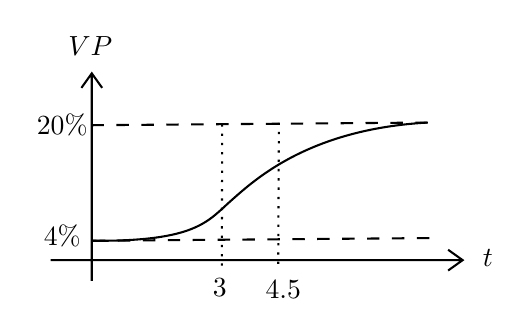
\begin{tikzpicture}[x=0.75pt,y=0.75pt,yscale=-1,xscale=1]
%uncomment if require: \path (0,300); %set diagram left start at 0, and has height of 300

%Shape: Axis 2D [id:dp8434144691544803] 
\draw  (171.87,196) -- (370.4,196)(191.72,106) -- (191.72,206) (363.4,191) -- (370.4,196) -- (363.4,201) (186.72,113) -- (191.72,106) -- (196.72,113)  ;
%Curve Lines [id:da3393494842698659] 
\draw    (192.33,186.67) .. controls (242.17,187) and (247.5,177.33) .. (258.83,167.33) .. controls (270.17,157.33) and (296.17,133) .. (353.17,129.73) ;


%Straight Lines [id:da6828905031101673] 
\draw  [dash pattern={on 4.5pt off 4.5pt}]  (191.6,131) -- (358,129.67) ;


%Straight Lines [id:da012395283086218845] 
\draw  [dash pattern={on 4.5pt off 4.5pt}]  (192.33,186.67) -- (358.73,185.33) ;


%Straight Lines [id:da9569907625895342] 
\draw  [dash pattern={on 0.84pt off 2.51pt}]  (281.87,129.73) -- (281.54,197.98) ;


%Straight Lines [id:da25982411660347404] 
\draw  [dash pattern={on 0.84pt off 2.51pt}]  (254.53,130.53) -- (254.39,200.06) ;


%%Straight Lines [id:da022260850258795317] 
%\draw    (160.2,170.6) -- (253.8,170.6) ;
%
%
%%Straight Lines [id:da5039184027623409] 
%\draw [line width=0.75]    (161,149.4) -- (282.6,149.4) ;



% Text Node
\draw (382.6,195.2) node   {$t$};
% Text Node
\draw (191,93) node   {$VP$};
% Text Node
\draw (177.5,131) node   {$20\%$};
% Text Node
\draw (177.5,184.5) node   {$4\%$};
% Text Node
\draw (253.4,209) node   {\SI{3}{\second}};
% Text Node
\draw (284,210) node   {\SI{4.5}{\second}};
%% Text Node
%\draw (135,145.5) node   {$0.632VP$};
%% Text Node
%\draw (135,168.5) node   {$0.283VP$};


\end{tikzpicture}
}
	\end{minipage}

	\vspace{1cm}

	\centering

	\Large
	Sistema instável
\end{frame}


\begin{frame}{Estabilidade}
	\begin{minipage}{0.49\linewidth}
		\centering
		\scalebox{0.8}{

\tikzset{every picture/.style={line width=0.75pt}} %set default line width to 0.75pt        

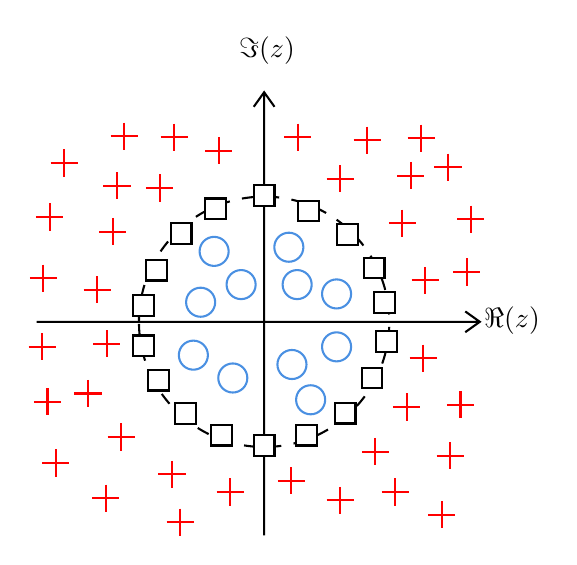
\begin{tikzpicture}[x=0.75pt,y=0.75pt,yscale=-1,xscale=1]
%uncomment if require: \path (0,300); %set diagram left start at 0, and has height of 300

%Shape: Circle [id:dp8434328262509021] 
\draw  [dash pattern={on 4.5pt off 4.5pt}] (89.28,160.6) .. controls (89.28,127.29) and (116.29,100.28) .. (149.6,100.28) .. controls (182.91,100.28) and (209.92,127.29) .. (209.92,160.6) .. controls (209.92,193.91) and (182.91,220.92) .. (149.6,220.92) .. controls (116.29,220.92) and (89.28,193.91) .. (89.28,160.6) -- cycle ;
%Shape: Axis 2D [id:dp27678030181731494] 
\draw  (40,160.6) -- (253.5,160.6)(149.6,50) -- (149.6,263.5) (246.5,155.6) -- (253.5,160.6) -- (246.5,165.6) (144.6,57) -- (149.6,50) -- (154.6,57)  ;
%Shape: Square [id:dp29640104318485094] 
\draw  [fill={rgb, 255:red, 255; green, 255; blue, 255 }  ,fill opacity=1 ] (183.6,199.6) -- (193.6,199.6) -- (193.6,209.6) -- (183.6,209.6) -- cycle ;
%Shape: Square [id:dp5015049228757054] 
\draw  [fill={rgb, 255:red, 255; green, 255; blue, 255 }  ,fill opacity=1 ] (166.1,102.2) -- (176.1,102.2) -- (176.1,112.2) -- (166.1,112.2) -- cycle ;
%Shape: Square [id:dp5724308304859749] 
\draw  [fill={rgb, 255:red, 255; green, 255; blue, 255 }  ,fill opacity=1 ] (144.6,94.7) -- (154.6,94.7) -- (154.6,104.7) -- (144.6,104.7) -- cycle ;
%Shape: Square [id:dp8722658997981245] 
\draw  [fill={rgb, 255:red, 255; green, 255; blue, 255 }  ,fill opacity=1 ] (184.6,113.7) -- (194.6,113.7) -- (194.6,123.7) -- (184.6,123.7) -- cycle ;
%Shape: Square [id:dp035501458242915174] 
\draw  [fill={rgb, 255:red, 255; green, 255; blue, 255 }  ,fill opacity=1 ] (165.1,210.2) -- (175.1,210.2) -- (175.1,220.2) -- (165.1,220.2) -- cycle ;
%Shape: Square [id:dp23226558696093957] 
\draw  [fill={rgb, 255:red, 255; green, 255; blue, 255 }  ,fill opacity=1 ] (144.6,215.2) -- (154.6,215.2) -- (154.6,225.2) -- (144.6,225.2) -- cycle ;
%Shape: Square [id:dp09667812864869552] 
\draw  [fill={rgb, 255:red, 255; green, 255; blue, 255 }  ,fill opacity=1 ] (106.6,199.7) -- (116.6,199.7) -- (116.6,209.7) -- (106.6,209.7) -- cycle ;
\draw  [color={rgb, 255:red, 255; green, 0; blue, 0 }  ,draw opacity=1 ] (159.17,71.63) -- (172.25,71.63)(165.71,65.08) -- (165.71,78.17) ;
%Shape: Circle [id:dp476022910470574] 
\draw  [color={rgb, 255:red, 74; green, 144; blue, 226 }  ,draw opacity=1 ] (118.5,126.67) .. controls (118.5,122.8) and (121.63,119.67) .. (125.5,119.67) .. controls (129.37,119.67) and (132.5,122.8) .. (132.5,126.67) .. controls (132.5,130.53) and (129.37,133.67) .. (125.5,133.67) .. controls (121.63,133.67) and (118.5,130.53) .. (118.5,126.67) -- cycle ;
\draw  [color={rgb, 255:red, 255; green, 0; blue, 0 }  ,draw opacity=1 ] (179.67,91.63) -- (192.75,91.63)(186.21,85.08) -- (186.21,98.17) ;
\draw  [color={rgb, 255:red, 255; green, 0; blue, 0 }  ,draw opacity=1 ] (209.67,113.13) -- (222.75,113.13)(216.21,106.58) -- (216.21,119.67) ;
\draw  [color={rgb, 255:red, 255; green, 0; blue, 0 }  ,draw opacity=1 ] (220.67,140.63) -- (233.75,140.63)(227.21,134.08) -- (227.21,147.17) ;
\draw  [color={rgb, 255:red, 255; green, 0; blue, 0 }  ,draw opacity=1 ] (219.67,178.13) -- (232.75,178.13)(226.21,171.58) -- (226.21,184.67) ;
\draw  [color={rgb, 255:red, 255; green, 0; blue, 0 }  ,draw opacity=1 ] (237.67,200.63) -- (250.75,200.63)(244.21,194.08) -- (244.21,207.17) ;
\draw  [color={rgb, 255:red, 255; green, 0; blue, 0 }  ,draw opacity=1 ] (232.67,225.13) -- (245.75,225.13)(239.21,218.58) -- (239.21,231.67) ;
\draw  [color={rgb, 255:red, 255; green, 0; blue, 0 }  ,draw opacity=1 ] (156.17,237.13) -- (169.25,237.13)(162.71,230.58) -- (162.71,243.67) ;
\draw  [color={rgb, 255:red, 255; green, 0; blue, 0 }  ,draw opacity=1 ] (126.67,242.63) -- (139.75,242.63)(133.21,236.08) -- (133.21,249.17) ;
\draw  [color={rgb, 255:red, 255; green, 0; blue, 0 }  ,draw opacity=1 ] (98.67,234.13) -- (111.75,234.13)(105.21,227.58) -- (105.21,240.67) ;
\draw  [color={rgb, 255:red, 255; green, 0; blue, 0 }  ,draw opacity=1 ] (74.17,216.13) -- (87.25,216.13)(80.71,209.58) -- (80.71,222.67) ;
\draw  [color={rgb, 255:red, 255; green, 0; blue, 0 }  ,draw opacity=1 ] (36.17,172.63) -- (49.25,172.63)(42.71,166.08) -- (42.71,179.17) ;
\draw  [color={rgb, 255:red, 255; green, 0; blue, 0 }  ,draw opacity=1 ] (62.67,145.13) -- (75.75,145.13)(69.21,138.58) -- (69.21,151.67) ;
\draw  [color={rgb, 255:red, 255; green, 0; blue, 0 }  ,draw opacity=1 ] (70.17,117.13) -- (83.25,117.13)(76.71,110.58) -- (76.71,123.67) ;
\draw  [color={rgb, 255:red, 255; green, 0; blue, 0 }  ,draw opacity=1 ] (46.67,84.13) -- (59.75,84.13)(53.21,77.58) -- (53.21,90.67) ;
\draw  [color={rgb, 255:red, 255; green, 0; blue, 0 }  ,draw opacity=1 ] (121.17,78.13) -- (134.25,78.13)(127.71,71.58) -- (127.71,84.67) ;
%Shape: Square [id:dp4796258381107217] 
\draw  [fill={rgb, 255:red, 255; green, 255; blue, 255 }  ,fill opacity=1 ] (197.6,129.7) -- (207.6,129.7) -- (207.6,139.7) -- (197.6,139.7) -- cycle ;
%Shape: Square [id:dp9590843867357357] 
\draw  [fill={rgb, 255:red, 255; green, 255; blue, 255 }  ,fill opacity=1 ] (202.6,146.2) -- (212.6,146.2) -- (212.6,156.2) -- (202.6,156.2) -- cycle ;
%Shape: Square [id:dp964054149374244] 
\draw  [fill={rgb, 255:red, 255; green, 255; blue, 255 }  ,fill opacity=1 ] (203.6,165.2) -- (213.6,165.2) -- (213.6,175.2) -- (203.6,175.2) -- cycle ;
%Shape: Square [id:dp7382656558458347] 
\draw  [fill={rgb, 255:red, 255; green, 255; blue, 255 }  ,fill opacity=1 ] (196.6,182.7) -- (206.6,182.7) -- (206.6,192.7) -- (196.6,192.7) -- cycle ;
%Shape: Square [id:dp21604742505805397] 
\draw  [fill={rgb, 255:red, 255; green, 255; blue, 255 }  ,fill opacity=1 ] (124.1,210.2) -- (134.1,210.2) -- (134.1,220.2) -- (124.1,220.2) -- cycle ;
%Shape: Square [id:dp8253346408417206] 
\draw  [fill={rgb, 255:red, 255; green, 255; blue, 255 }  ,fill opacity=1 ] (93.6,183.7) -- (103.6,183.7) -- (103.6,193.7) -- (93.6,193.7) -- cycle ;
%Shape: Square [id:dp3602080753175103] 
\draw  [fill={rgb, 255:red, 255; green, 255; blue, 255 }  ,fill opacity=1 ] (86.6,167.2) -- (96.6,167.2) -- (96.6,177.2) -- (86.6,177.2) -- cycle ;
%Shape: Square [id:dp7299074290585237] 
\draw  [fill={rgb, 255:red, 255; green, 255; blue, 255 }  ,fill opacity=1 ] (86.6,147.7) -- (96.6,147.7) -- (96.6,157.7) -- (86.6,157.7) -- cycle ;
%Shape: Square [id:dp3870669064913592] 
\draw  [fill={rgb, 255:red, 255; green, 255; blue, 255 }  ,fill opacity=1 ] (92.6,130.7) -- (102.6,130.7) -- (102.6,140.7) -- (92.6,140.7) -- cycle ;
%Shape: Square [id:dp0778563841598956] 
\draw  [fill={rgb, 255:red, 255; green, 255; blue, 255 }  ,fill opacity=1 ] (104.6,113.2) -- (114.6,113.2) -- (114.6,123.2) -- (104.6,123.2) -- cycle ;
%Shape: Square [id:dp4833937813802225] 
\draw  [fill={rgb, 255:red, 255; green, 255; blue, 255 }  ,fill opacity=1 ] (121.1,101.2) -- (131.1,101.2) -- (131.1,111.2) -- (121.1,111.2) -- cycle ;
%Shape: Circle [id:dp22437252791244577] 
\draw  [color={rgb, 255:red, 74; green, 144; blue, 226 }  ,draw opacity=1 ] (154.5,124.67) .. controls (154.5,120.8) and (157.63,117.67) .. (161.5,117.67) .. controls (165.37,117.67) and (168.5,120.8) .. (168.5,124.67) .. controls (168.5,128.53) and (165.37,131.67) .. (161.5,131.67) .. controls (157.63,131.67) and (154.5,128.53) .. (154.5,124.67) -- cycle ;
%Shape: Circle [id:dp4682090317035761] 
\draw  [color={rgb, 255:red, 74; green, 144; blue, 226 }  ,draw opacity=1 ] (177.5,147.17) .. controls (177.5,143.3) and (180.63,140.17) .. (184.5,140.17) .. controls (188.37,140.17) and (191.5,143.3) .. (191.5,147.17) .. controls (191.5,151.03) and (188.37,154.17) .. (184.5,154.17) .. controls (180.63,154.17) and (177.5,151.03) .. (177.5,147.17) -- cycle ;
%Shape: Circle [id:dp006880258312718768] 
\draw  [color={rgb, 255:red, 74; green, 144; blue, 226 }  ,draw opacity=1 ] (177.5,172.67) .. controls (177.5,168.8) and (180.63,165.67) .. (184.5,165.67) .. controls (188.37,165.67) and (191.5,168.8) .. (191.5,172.67) .. controls (191.5,176.53) and (188.37,179.67) .. (184.5,179.67) .. controls (180.63,179.67) and (177.5,176.53) .. (177.5,172.67) -- cycle ;
%Shape: Circle [id:dp6362725623770331] 
\draw  [color={rgb, 255:red, 74; green, 144; blue, 226 }  ,draw opacity=1 ] (156,181.17) .. controls (156,177.3) and (159.13,174.17) .. (163,174.17) .. controls (166.87,174.17) and (170,177.3) .. (170,181.17) .. controls (170,185.03) and (166.87,188.17) .. (163,188.17) .. controls (159.13,188.17) and (156,185.03) .. (156,181.17) -- cycle ;
%Shape: Circle [id:dp80425166884741] 
\draw  [color={rgb, 255:red, 74; green, 144; blue, 226 }  ,draw opacity=1 ] (158.5,142.67) .. controls (158.5,138.8) and (161.63,135.67) .. (165.5,135.67) .. controls (169.37,135.67) and (172.5,138.8) .. (172.5,142.67) .. controls (172.5,146.53) and (169.37,149.67) .. (165.5,149.67) .. controls (161.63,149.67) and (158.5,146.53) .. (158.5,142.67) -- cycle ;
%Shape: Circle [id:dp5115888880559238] 
\draw  [color={rgb, 255:red, 74; green, 144; blue, 226 }  ,draw opacity=1 ] (131.5,142.67) .. controls (131.5,138.8) and (134.63,135.67) .. (138.5,135.67) .. controls (142.37,135.67) and (145.5,138.8) .. (145.5,142.67) .. controls (145.5,146.53) and (142.37,149.67) .. (138.5,149.67) .. controls (134.63,149.67) and (131.5,146.53) .. (131.5,142.67) -- cycle ;
%Shape: Circle [id:dp9193079828474959] 
\draw  [color={rgb, 255:red, 74; green, 144; blue, 226 }  ,draw opacity=1 ] (112,151.17) .. controls (112,147.3) and (115.13,144.17) .. (119,144.17) .. controls (122.87,144.17) and (126,147.3) .. (126,151.17) .. controls (126,155.03) and (122.87,158.17) .. (119,158.17) .. controls (115.13,158.17) and (112,155.03) .. (112,151.17) -- cycle ;
%Shape: Circle [id:dp33233029245659296] 
\draw  [color={rgb, 255:red, 74; green, 144; blue, 226 }  ,draw opacity=1 ] (108.5,176.67) .. controls (108.5,172.8) and (111.63,169.67) .. (115.5,169.67) .. controls (119.37,169.67) and (122.5,172.8) .. (122.5,176.67) .. controls (122.5,180.53) and (119.37,183.67) .. (115.5,183.67) .. controls (111.63,183.67) and (108.5,180.53) .. (108.5,176.67) -- cycle ;
%Shape: Circle [id:dp3198604312654221] 
\draw  [color={rgb, 255:red, 74; green, 144; blue, 226 }  ,draw opacity=1 ] (127.5,187.67) .. controls (127.5,183.8) and (130.63,180.67) .. (134.5,180.67) .. controls (138.37,180.67) and (141.5,183.8) .. (141.5,187.67) .. controls (141.5,191.53) and (138.37,194.67) .. (134.5,194.67) .. controls (130.63,194.67) and (127.5,191.53) .. (127.5,187.67) -- cycle ;
%Shape: Circle [id:dp5700084778547776] 
\draw  [color={rgb, 255:red, 74; green, 144; blue, 226 }  ,draw opacity=1 ] (165,198.17) .. controls (165,194.3) and (168.13,191.17) .. (172,191.17) .. controls (175.87,191.17) and (179,194.3) .. (179,198.17) .. controls (179,202.03) and (175.87,205.17) .. (172,205.17) .. controls (168.13,205.17) and (165,202.03) .. (165,198.17) -- cycle ;
\draw  [color={rgb, 255:red, 255; green, 0; blue, 0 }  ,draw opacity=1 ] (240.67,136.63) -- (253.75,136.63)(247.21,130.08) -- (247.21,143.17) ;
\draw  [color={rgb, 255:red, 255; green, 0; blue, 0 }  ,draw opacity=1 ] (242.67,111.13) -- (255.75,111.13)(249.21,104.58) -- (249.21,117.67) ;
\draw  [color={rgb, 255:red, 255; green, 0; blue, 0 }  ,draw opacity=1 ] (231.67,86.13) -- (244.75,86.13)(238.21,79.58) -- (238.21,92.67) ;
\draw  [color={rgb, 255:red, 255; green, 0; blue, 0 }  ,draw opacity=1 ] (213.67,90.13) -- (226.75,90.13)(220.21,83.58) -- (220.21,96.67) ;
\draw  [color={rgb, 255:red, 255; green, 0; blue, 0 }  ,draw opacity=1 ] (192.67,73.13) -- (205.75,73.13)(199.21,66.58) -- (199.21,79.67) ;
\draw  [color={rgb, 255:red, 255; green, 0; blue, 0 }  ,draw opacity=1 ] (218.67,72.13) -- (231.75,72.13)(225.21,65.58) -- (225.21,78.67) ;
\draw  [color={rgb, 255:red, 255; green, 0; blue, 0 }  ,draw opacity=1 ] (99.67,71.63) -- (112.75,71.63)(106.21,65.08) -- (106.21,78.17) ;
\draw  [color={rgb, 255:red, 255; green, 0; blue, 0 }  ,draw opacity=1 ] (92.67,96.13) -- (105.75,96.13)(99.21,89.58) -- (99.21,102.67) ;
\draw  [color={rgb, 255:red, 255; green, 0; blue, 0 }  ,draw opacity=1 ] (36.67,139.63) -- (49.75,139.63)(43.21,133.08) -- (43.21,146.17) ;
\draw  [color={rgb, 255:red, 255; green, 0; blue, 0 }  ,draw opacity=1 ] (72.17,95.13) -- (85.25,95.13)(78.71,88.58) -- (78.71,101.67) ;
\draw  [color={rgb, 255:red, 255; green, 0; blue, 0 }  ,draw opacity=1 ] (75.67,71.13) -- (88.75,71.13)(82.21,64.58) -- (82.21,77.67) ;
\draw  [color={rgb, 255:red, 255; green, 0; blue, 0 }  ,draw opacity=1 ] (39.67,110.13) -- (52.75,110.13)(46.21,103.58) -- (46.21,116.67) ;
\draw  [color={rgb, 255:red, 255; green, 0; blue, 0 }  ,draw opacity=1 ] (58.17,195.13) -- (71.25,195.13)(64.71,188.58) -- (64.71,201.67) ;
\draw  [color={rgb, 255:red, 255; green, 0; blue, 0 }  ,draw opacity=1 ] (102.67,257.13) -- (115.75,257.13)(109.21,250.58) -- (109.21,263.67) ;
\draw  [color={rgb, 255:red, 255; green, 0; blue, 0 }  ,draw opacity=1 ] (66.67,245.63) -- (79.75,245.63)(73.21,239.08) -- (73.21,252.17) ;
\draw  [color={rgb, 255:red, 255; green, 0; blue, 0 }  ,draw opacity=1 ] (42.67,228.63) -- (55.75,228.63)(49.21,222.08) -- (49.21,235.17) ;
\draw  [color={rgb, 255:red, 255; green, 0; blue, 0 }  ,draw opacity=1 ] (38.67,199.13) -- (51.75,199.13)(45.21,192.58) -- (45.21,205.67) ;
\draw  [color={rgb, 255:red, 255; green, 0; blue, 0 }  ,draw opacity=1 ] (67.17,171.13) -- (80.25,171.13)(73.71,164.58) -- (73.71,177.67) ;
\draw  [color={rgb, 255:red, 255; green, 0; blue, 0 }  ,draw opacity=1 ] (206.17,242.63) -- (219.25,242.63)(212.71,236.08) -- (212.71,249.17) ;
\draw  [color={rgb, 255:red, 255; green, 0; blue, 0 }  ,draw opacity=1 ] (228.67,253.63) -- (241.75,253.63)(235.21,247.08) -- (235.21,260.17) ;
\draw  [color={rgb, 255:red, 255; green, 0; blue, 0 }  ,draw opacity=1 ] (196.67,223.13) -- (209.75,223.13)(203.21,216.58) -- (203.21,229.67) ;
\draw  [color={rgb, 255:red, 255; green, 0; blue, 0 }  ,draw opacity=1 ] (211.67,201.63) -- (224.75,201.63)(218.21,195.08) -- (218.21,208.17) ;
\draw  [color={rgb, 255:red, 255; green, 0; blue, 0 }  ,draw opacity=1 ] (179.67,246.63) -- (192.75,246.63)(186.21,240.08) -- (186.21,253.17) ;

% Text Node
\draw (151,30) node   {$\Im(z)$};
% Text Node
\draw (269,160) node   {$\Re(z)$};


\end{tikzpicture}
}
		
		\medskip
		
		Sistema estável
	\end{minipage}
	\hfill
	\begin{minipage}{0.49\linewidth}
		\centering
		
		\vspace{1.6cm}
		\scalebox{1.2}{\begin{tikzpicture}
	\draw[->] (-2.5,0) -- (2.5,0) node[right] {$ \sigma $};
	\draw[->] (0,-2) -- (0,2) node[above] {$ j\omega $};
	
	\draw (0,0) node[below left] {$ 0 $};
	
	\draw (-1,-2) -- (-1,2) (1,-2) -- (1,2);
	
	\node [above left] at (-1,0) {$ -\sigma_1 $};
	\node [above right] at (1,0) {$ \sigma_2 $};
\end{tikzpicture}}
		
		\medskip
		
		Sistema instável
	\end{minipage}
	
	\vspace{1cm}
	
	\centering
	
	\Large
	
\end{frame}


%\begin{frame}{Estabilidade}
%	\begin{block}{BIBO estabilidade}
%		\begin{itemize}
%			\item Um sistema é BIBO (\textit{Bounded-Input, Bounded-Output}) estável se ele possui uma saída que é limitada tal qual sua entrada.
%		\end{itemize}
%	\end{block}
%
%	\vspace{0.3cm}
%	\begin{minipage}{0.49\linewidth}
%		\centering
%		
%		\scalebox{0.9}{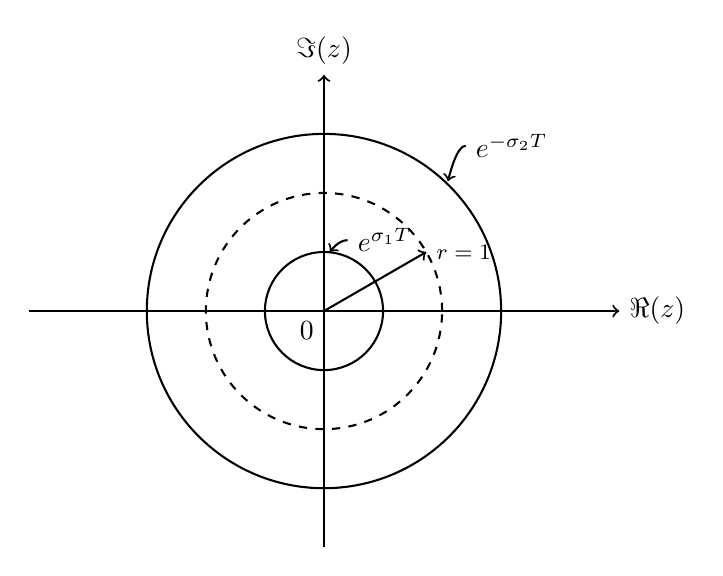
\begin{tikzpicture}[scale=1.5]
	\draw[->] (-2.5,0) -- (2.5,0) node[right] {$ \Re(z) $};
	\draw[->] (0,-2) -- (0,2) node[above] {$ \Im(z) $};
	
	\draw (0,0) circle (1.5);
	\draw[dashed] (0,0) circle (1);
	\draw (0,0) circle (0.5);
	
%	\node [below left] at (-1,0) {$ -1 $};
%	\node [below right] at (0,-1) {$ -1 $};
%	\node [above right] at (0,1) {$ 1 $};
%	\node [below right] at (1,0) {$ 1 $};

	\draw (0,0) node[below left] {$ 0 $};
	
	\draw [->] (0.2, 0.6) node[right] {$ \text{e}^{\sigma_1T} $} parabola (0.05,0.5);
	
	\draw [->] (1.2, 1.4) node[right] {$ \text{e}^{-\sigma_2T} $} parabola (1.05,1.1);
	
	\draw[->] (0,0) -- (30:1) node[right=0pt] {\footnotesize $ r=1 $};
\end{tikzpicture}}
%	\end{minipage}
%	\hfill
%	\begin{minipage}{0.49\linewidth}
%		\centering
%		
%		\scalebox{0.9}{

\tikzset{every picture/.style={line width=0.75pt}} %set default line width to 0.75pt        

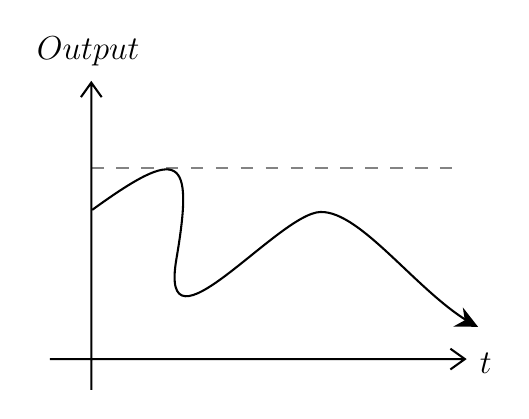
\begin{tikzpicture}[x=0.75pt,y=0.75pt,yscale=-1,xscale=1]
%uncomment if require: \path (0,300); %set diagram left start at 0, and has height of 300

%Straight Lines [id:da45173516768188793] 
\draw [color={rgb, 255:red, 131; green, 131; blue, 131 }  ,draw opacity=1 ] [dash pattern={on 4.5pt off 4.5pt}]  (110,131.33) -- (290,131.33) ;


%Shape: Axis 2D [id:dp17702348361548204] 
\draw  (90,223.2) -- (290,223.2)(110,90) -- (110,238) (283,218.2) -- (290,223.2) -- (283,228.2) (105,97) -- (110,90) -- (115,97)  ;
%Curve Lines [id:da6473783232781454] 
\draw    (110.42,151.33) .. controls (152.75,120.66) and (159.67,124.33) .. (151,174.99) .. controls (142.33,225.66) and (200,152.99) .. (220.33,152.33) .. controls (240.26,151.67) and (268.19,192.64) .. (294.71,206.83) ;
\draw [shift={(296.33,207.66)}, rotate = 206.28] [fill={rgb, 255:red, 0; green, 0; blue, 0 }  ][line width=0.75]  [draw opacity=0] (10.72,-5.15) -- (0,0) -- (10.72,5.15) -- (7.12,0) -- cycle    ;


% Text Node
\draw (108.5,75) node   {\large $Output$};
% Text Node
\draw (300,225) node   {\large $t$};


\end{tikzpicture}
}
%	\end{minipage}
%\end{frame}


\begin{frame}{Conceitos preliminares}
	\begin{block}{Processo}
		\begin{itemize}
			\item Um \textbf{processo} é qualquer atividade (ou conjunto de atividades) que tem algum \textbf{objetivo}.
		\end{itemize}
	\end{block}

	\vspace{0.5cm}

	\begin{minipage}{0.49\linewidth}
		\centering
		\includegraphics[width=1\linewidth]{Figuras/Ch11/fig3}
	\end{minipage}
	\hfill
	\begin{minipage}{0.49\linewidth}
		\centering
		\includegraphics[width=1\linewidth]{Figuras/Ch11/fig4}
	\end{minipage}
\end{frame}


\begin{frame}{Conceitos preliminares}
	\begin{block}{Variáveis de processo}
		\begin{itemize}
			\item As \textbf{variáveis de processo} são aquelas \textbf{envolvidas no processo}.
			\item Estas podem ser alteradas durante o processo, e podem ser usadas para \textbf{medir os resultados} e/ou \textbf{controlá-los}.
		\end{itemize}
	\end{block}
	
%	\vspace{0.5cm}
	
	\centering
	\includegraphics[width=0.8\linewidth]{Figuras/Ch11/fig5}
\end{frame}


\begin{frame}{Conceitos preliminares}
	\begin{block}{Outras variáveis e \textit{setpoint}}
		\begin{itemize}
			\item O \textbf{controle de processos} vai ajustar uma \textbf{variável manipulada} e, assim, estabilizar a \textbf{variável controlada} em seu \textbf{\textit{setpoint}}.
		\end{itemize}
	\end{block}
	
	%	\vspace{0.5cm}
	
	\centering
	\includegraphics[width=0.8\linewidth]{Figuras/Ch11/fig6}
\end{frame}


\begin{frame}{Malha aberta x malha fechada}
	\begin{block}{Introdução}
		\begin{itemize}
			\item O controle de malha aberta pode ser suficiente em vários sistemas onde as condições de operação são \textbf{constantes}, mas e se não forem?
		\end{itemize}
	\end{block}
	
	%	\vspace{0.5cm}
	
	\centering
	\includegraphics[height=0.65\textheight]{Figuras/Ch11/fig7}
\end{frame}


\begin{frame}{Malha aberta x malha fechada}
	\begin{block}{Diagramas de blocos}
		\begin{itemize}
			\item Os diagramas de blocos nos ajudam a compreender o funcionamento das malhas, indicando cada componente e sua função na malha.
		\end{itemize}
	\end{block}
	
	\vspace{1cm}
	
	\centering
	\deftkzbds
	\begin{tikzpicture}[auto, node distance=2cm,>=Latex]
	\node[input] (in) {};
	\node[block, right=of in] (B) {Bloco};
	\node[output,right=of B] (out) {}; 
	
	\draw[->] (in) -- node[above,midway] {Entrada} (B);
	\draw[->] (B) -- node[above,midway] {Saída} (out);
	\end{tikzpicture}
\end{frame}


\begin{frame}{Malha aberta x malha fechada}
	\begin{block}{Malha aberta}
		\begin{itemize}
			\item Uma \textbf{malha aberta} pode ser mostrada por um diagrama de blocos com apenas dois elementos.
			\item A malha aberta pode lidar com \textbf{quaisquer problemas já conhecidos}, pois já são contados em seu \textbf{funcionamento normal}.
		\end{itemize}
	\end{block}
	
	\vspace{1cm}
	
	\centering
	\deftkzbds
	\begin{tikzpicture}[auto, node distance=2cm,>=Latex]
	\node[input] (in) {};
	\node[block, right=of in] (C) {Controlador};
	\node[block, right=of C] (P) {Processo};
	\node[output,right=of P] (out) {}; 
	
	\draw[->] (in) -- node[above,midway] {Entrada} (C);
	\draw[->] (C) -- (P);
	\draw[->] (P) -- (out) node[above,midway] {Saída};
	\end{tikzpicture}
\end{frame}


\begin{frame}{Malha aberta x malha fechada}
	\begin{block}{Malha fechada}
		A malha fechada conta com alguns componentes adicionais, entre eles:
		\begin{itemize}
			\item \textbf{Comparador}
			
			Compara o valor de \textbf{referência} com o \textbf{valor medido} na saída e gera um sinal de \textbf{erro} que indica o quanto o sinal de saída está longe do sinal de entrada.
			\item \textbf{Atuador}
			
			A partir do sinal recebido do controlador, atua sobre a \textbf{variável manipulada} para ajustar e alterar a variável controlada de modo a \textbf{corrigir o erro}.
			\item \textbf{Sensor}
			
			\textbf{Lê a variável controlada} na saída e envia sua condição na forma de sinal para o comparador, fechando o laço.
		\end{itemize}
	\end{block}
\end{frame}


\begin{frame}{Malha aberta x malha fechada}
	\begin{block}{Malha fechada}
		\begin{itemize}
			\item Os componentes da malha fechada devem regular sua saída \textbf{independentemente} das condições do processo.
			\item O sensor deverá \textbf{ler a saída} e \textbf{enviar seu sinal} (através de um transmissor) para o comparador, que deve enviar o \textbf{erro} para o controlador.
			\item O controlador, então, deve enviar um sinal calculado (ao atuador) para \textbf{corrigir} a saída do processo, que deve tender ao \textbf{valor desejado} (\textit{setpoint}).
		\end{itemize}
	\end{block}

%	\vspace{0.5cm}
	
	\centering
	\scalebox{0.7}{
		\deftkzbds
		\begin{tikzpicture}[auto, node distance=1cm,>=Latex]
			\node[input] (in) {};
			\node[sum,right=1.5cm of in] (sum) {\Large $ + $};
			\node[block, right=of sum] (C) {Controlador};
			\node[block,right=of C] (A) {Atuador};
			\node[block, right=of A] (P) {Processo};
			\coordinate[right=of P] (mid);
			\node[output,right=of mid] (out) {};
			\node[block,below=of A] (S) {Sensor};
			
			\draw[->] (in) -- node[above,midway] {Entrada} (sum) node[above=12pt] {Comparador};
			\draw[->] (sum) -- (C);
			\draw[->] (C) -- (A);
			\draw[->] (A) -- (P);
			\draw[->] (mid) |- (S);
			\draw[->] (S) -| node[pos=0.98, xshift=15pt] {$-$} node[pos=1.19, xshift=-4pt] {$+$} (sum);
			\draw[->] (P) -- (out) node[above,near end] {Saída};
		\end{tikzpicture}}
\end{frame}


\begin{frame}{Correção da saída}
	\begin{block}{Introdução}
		\begin{itemize}
			\item Assim que é detectada uma \textbf{anormalidade} na saída, isto é, um \textbf{erro}, em uma malha fechada, o controlador deve responder para corrigí-lo.
			\item Se o erro for \textbf{muito grande}, a resposta do controlador pode ser \textbf{muito drástica}, causando um erro \textbf{tão grande quanto}, mas \textbf{oposto} ao original.
		\end{itemize}
	\end{block}

	\vspace{-1.5cm}

	\centering
	\scalebox{0.8}{

\tikzset{every picture/.style={line width=0.75pt}} %set default line width to 0.75pt        

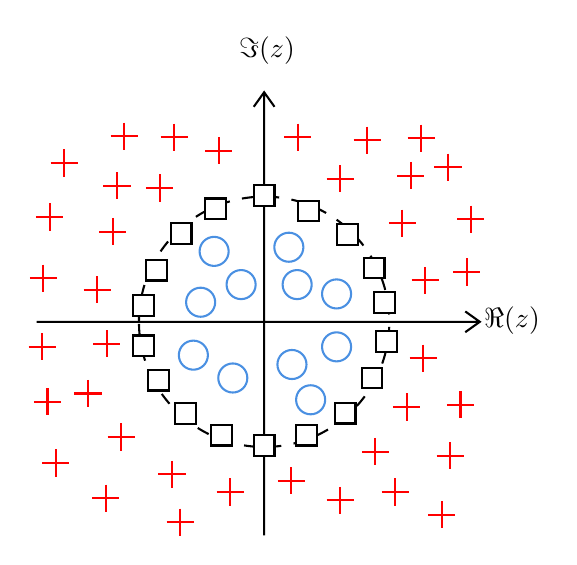
\begin{tikzpicture}[x=0.75pt,y=0.75pt,yscale=-1,xscale=1]
%uncomment if require: \path (0,300); %set diagram left start at 0, and has height of 300

%Shape: Circle [id:dp8434328262509021] 
\draw  [dash pattern={on 4.5pt off 4.5pt}] (89.28,160.6) .. controls (89.28,127.29) and (116.29,100.28) .. (149.6,100.28) .. controls (182.91,100.28) and (209.92,127.29) .. (209.92,160.6) .. controls (209.92,193.91) and (182.91,220.92) .. (149.6,220.92) .. controls (116.29,220.92) and (89.28,193.91) .. (89.28,160.6) -- cycle ;
%Shape: Axis 2D [id:dp27678030181731494] 
\draw  (40,160.6) -- (253.5,160.6)(149.6,50) -- (149.6,263.5) (246.5,155.6) -- (253.5,160.6) -- (246.5,165.6) (144.6,57) -- (149.6,50) -- (154.6,57)  ;
%Shape: Square [id:dp29640104318485094] 
\draw  [fill={rgb, 255:red, 255; green, 255; blue, 255 }  ,fill opacity=1 ] (183.6,199.6) -- (193.6,199.6) -- (193.6,209.6) -- (183.6,209.6) -- cycle ;
%Shape: Square [id:dp5015049228757054] 
\draw  [fill={rgb, 255:red, 255; green, 255; blue, 255 }  ,fill opacity=1 ] (166.1,102.2) -- (176.1,102.2) -- (176.1,112.2) -- (166.1,112.2) -- cycle ;
%Shape: Square [id:dp5724308304859749] 
\draw  [fill={rgb, 255:red, 255; green, 255; blue, 255 }  ,fill opacity=1 ] (144.6,94.7) -- (154.6,94.7) -- (154.6,104.7) -- (144.6,104.7) -- cycle ;
%Shape: Square [id:dp8722658997981245] 
\draw  [fill={rgb, 255:red, 255; green, 255; blue, 255 }  ,fill opacity=1 ] (184.6,113.7) -- (194.6,113.7) -- (194.6,123.7) -- (184.6,123.7) -- cycle ;
%Shape: Square [id:dp035501458242915174] 
\draw  [fill={rgb, 255:red, 255; green, 255; blue, 255 }  ,fill opacity=1 ] (165.1,210.2) -- (175.1,210.2) -- (175.1,220.2) -- (165.1,220.2) -- cycle ;
%Shape: Square [id:dp23226558696093957] 
\draw  [fill={rgb, 255:red, 255; green, 255; blue, 255 }  ,fill opacity=1 ] (144.6,215.2) -- (154.6,215.2) -- (154.6,225.2) -- (144.6,225.2) -- cycle ;
%Shape: Square [id:dp09667812864869552] 
\draw  [fill={rgb, 255:red, 255; green, 255; blue, 255 }  ,fill opacity=1 ] (106.6,199.7) -- (116.6,199.7) -- (116.6,209.7) -- (106.6,209.7) -- cycle ;
\draw  [color={rgb, 255:red, 255; green, 0; blue, 0 }  ,draw opacity=1 ] (159.17,71.63) -- (172.25,71.63)(165.71,65.08) -- (165.71,78.17) ;
%Shape: Circle [id:dp476022910470574] 
\draw  [color={rgb, 255:red, 74; green, 144; blue, 226 }  ,draw opacity=1 ] (118.5,126.67) .. controls (118.5,122.8) and (121.63,119.67) .. (125.5,119.67) .. controls (129.37,119.67) and (132.5,122.8) .. (132.5,126.67) .. controls (132.5,130.53) and (129.37,133.67) .. (125.5,133.67) .. controls (121.63,133.67) and (118.5,130.53) .. (118.5,126.67) -- cycle ;
\draw  [color={rgb, 255:red, 255; green, 0; blue, 0 }  ,draw opacity=1 ] (179.67,91.63) -- (192.75,91.63)(186.21,85.08) -- (186.21,98.17) ;
\draw  [color={rgb, 255:red, 255; green, 0; blue, 0 }  ,draw opacity=1 ] (209.67,113.13) -- (222.75,113.13)(216.21,106.58) -- (216.21,119.67) ;
\draw  [color={rgb, 255:red, 255; green, 0; blue, 0 }  ,draw opacity=1 ] (220.67,140.63) -- (233.75,140.63)(227.21,134.08) -- (227.21,147.17) ;
\draw  [color={rgb, 255:red, 255; green, 0; blue, 0 }  ,draw opacity=1 ] (219.67,178.13) -- (232.75,178.13)(226.21,171.58) -- (226.21,184.67) ;
\draw  [color={rgb, 255:red, 255; green, 0; blue, 0 }  ,draw opacity=1 ] (237.67,200.63) -- (250.75,200.63)(244.21,194.08) -- (244.21,207.17) ;
\draw  [color={rgb, 255:red, 255; green, 0; blue, 0 }  ,draw opacity=1 ] (232.67,225.13) -- (245.75,225.13)(239.21,218.58) -- (239.21,231.67) ;
\draw  [color={rgb, 255:red, 255; green, 0; blue, 0 }  ,draw opacity=1 ] (156.17,237.13) -- (169.25,237.13)(162.71,230.58) -- (162.71,243.67) ;
\draw  [color={rgb, 255:red, 255; green, 0; blue, 0 }  ,draw opacity=1 ] (126.67,242.63) -- (139.75,242.63)(133.21,236.08) -- (133.21,249.17) ;
\draw  [color={rgb, 255:red, 255; green, 0; blue, 0 }  ,draw opacity=1 ] (98.67,234.13) -- (111.75,234.13)(105.21,227.58) -- (105.21,240.67) ;
\draw  [color={rgb, 255:red, 255; green, 0; blue, 0 }  ,draw opacity=1 ] (74.17,216.13) -- (87.25,216.13)(80.71,209.58) -- (80.71,222.67) ;
\draw  [color={rgb, 255:red, 255; green, 0; blue, 0 }  ,draw opacity=1 ] (36.17,172.63) -- (49.25,172.63)(42.71,166.08) -- (42.71,179.17) ;
\draw  [color={rgb, 255:red, 255; green, 0; blue, 0 }  ,draw opacity=1 ] (62.67,145.13) -- (75.75,145.13)(69.21,138.58) -- (69.21,151.67) ;
\draw  [color={rgb, 255:red, 255; green, 0; blue, 0 }  ,draw opacity=1 ] (70.17,117.13) -- (83.25,117.13)(76.71,110.58) -- (76.71,123.67) ;
\draw  [color={rgb, 255:red, 255; green, 0; blue, 0 }  ,draw opacity=1 ] (46.67,84.13) -- (59.75,84.13)(53.21,77.58) -- (53.21,90.67) ;
\draw  [color={rgb, 255:red, 255; green, 0; blue, 0 }  ,draw opacity=1 ] (121.17,78.13) -- (134.25,78.13)(127.71,71.58) -- (127.71,84.67) ;
%Shape: Square [id:dp4796258381107217] 
\draw  [fill={rgb, 255:red, 255; green, 255; blue, 255 }  ,fill opacity=1 ] (197.6,129.7) -- (207.6,129.7) -- (207.6,139.7) -- (197.6,139.7) -- cycle ;
%Shape: Square [id:dp9590843867357357] 
\draw  [fill={rgb, 255:red, 255; green, 255; blue, 255 }  ,fill opacity=1 ] (202.6,146.2) -- (212.6,146.2) -- (212.6,156.2) -- (202.6,156.2) -- cycle ;
%Shape: Square [id:dp964054149374244] 
\draw  [fill={rgb, 255:red, 255; green, 255; blue, 255 }  ,fill opacity=1 ] (203.6,165.2) -- (213.6,165.2) -- (213.6,175.2) -- (203.6,175.2) -- cycle ;
%Shape: Square [id:dp7382656558458347] 
\draw  [fill={rgb, 255:red, 255; green, 255; blue, 255 }  ,fill opacity=1 ] (196.6,182.7) -- (206.6,182.7) -- (206.6,192.7) -- (196.6,192.7) -- cycle ;
%Shape: Square [id:dp21604742505805397] 
\draw  [fill={rgb, 255:red, 255; green, 255; blue, 255 }  ,fill opacity=1 ] (124.1,210.2) -- (134.1,210.2) -- (134.1,220.2) -- (124.1,220.2) -- cycle ;
%Shape: Square [id:dp8253346408417206] 
\draw  [fill={rgb, 255:red, 255; green, 255; blue, 255 }  ,fill opacity=1 ] (93.6,183.7) -- (103.6,183.7) -- (103.6,193.7) -- (93.6,193.7) -- cycle ;
%Shape: Square [id:dp3602080753175103] 
\draw  [fill={rgb, 255:red, 255; green, 255; blue, 255 }  ,fill opacity=1 ] (86.6,167.2) -- (96.6,167.2) -- (96.6,177.2) -- (86.6,177.2) -- cycle ;
%Shape: Square [id:dp7299074290585237] 
\draw  [fill={rgb, 255:red, 255; green, 255; blue, 255 }  ,fill opacity=1 ] (86.6,147.7) -- (96.6,147.7) -- (96.6,157.7) -- (86.6,157.7) -- cycle ;
%Shape: Square [id:dp3870669064913592] 
\draw  [fill={rgb, 255:red, 255; green, 255; blue, 255 }  ,fill opacity=1 ] (92.6,130.7) -- (102.6,130.7) -- (102.6,140.7) -- (92.6,140.7) -- cycle ;
%Shape: Square [id:dp0778563841598956] 
\draw  [fill={rgb, 255:red, 255; green, 255; blue, 255 }  ,fill opacity=1 ] (104.6,113.2) -- (114.6,113.2) -- (114.6,123.2) -- (104.6,123.2) -- cycle ;
%Shape: Square [id:dp4833937813802225] 
\draw  [fill={rgb, 255:red, 255; green, 255; blue, 255 }  ,fill opacity=1 ] (121.1,101.2) -- (131.1,101.2) -- (131.1,111.2) -- (121.1,111.2) -- cycle ;
%Shape: Circle [id:dp22437252791244577] 
\draw  [color={rgb, 255:red, 74; green, 144; blue, 226 }  ,draw opacity=1 ] (154.5,124.67) .. controls (154.5,120.8) and (157.63,117.67) .. (161.5,117.67) .. controls (165.37,117.67) and (168.5,120.8) .. (168.5,124.67) .. controls (168.5,128.53) and (165.37,131.67) .. (161.5,131.67) .. controls (157.63,131.67) and (154.5,128.53) .. (154.5,124.67) -- cycle ;
%Shape: Circle [id:dp4682090317035761] 
\draw  [color={rgb, 255:red, 74; green, 144; blue, 226 }  ,draw opacity=1 ] (177.5,147.17) .. controls (177.5,143.3) and (180.63,140.17) .. (184.5,140.17) .. controls (188.37,140.17) and (191.5,143.3) .. (191.5,147.17) .. controls (191.5,151.03) and (188.37,154.17) .. (184.5,154.17) .. controls (180.63,154.17) and (177.5,151.03) .. (177.5,147.17) -- cycle ;
%Shape: Circle [id:dp006880258312718768] 
\draw  [color={rgb, 255:red, 74; green, 144; blue, 226 }  ,draw opacity=1 ] (177.5,172.67) .. controls (177.5,168.8) and (180.63,165.67) .. (184.5,165.67) .. controls (188.37,165.67) and (191.5,168.8) .. (191.5,172.67) .. controls (191.5,176.53) and (188.37,179.67) .. (184.5,179.67) .. controls (180.63,179.67) and (177.5,176.53) .. (177.5,172.67) -- cycle ;
%Shape: Circle [id:dp6362725623770331] 
\draw  [color={rgb, 255:red, 74; green, 144; blue, 226 }  ,draw opacity=1 ] (156,181.17) .. controls (156,177.3) and (159.13,174.17) .. (163,174.17) .. controls (166.87,174.17) and (170,177.3) .. (170,181.17) .. controls (170,185.03) and (166.87,188.17) .. (163,188.17) .. controls (159.13,188.17) and (156,185.03) .. (156,181.17) -- cycle ;
%Shape: Circle [id:dp80425166884741] 
\draw  [color={rgb, 255:red, 74; green, 144; blue, 226 }  ,draw opacity=1 ] (158.5,142.67) .. controls (158.5,138.8) and (161.63,135.67) .. (165.5,135.67) .. controls (169.37,135.67) and (172.5,138.8) .. (172.5,142.67) .. controls (172.5,146.53) and (169.37,149.67) .. (165.5,149.67) .. controls (161.63,149.67) and (158.5,146.53) .. (158.5,142.67) -- cycle ;
%Shape: Circle [id:dp5115888880559238] 
\draw  [color={rgb, 255:red, 74; green, 144; blue, 226 }  ,draw opacity=1 ] (131.5,142.67) .. controls (131.5,138.8) and (134.63,135.67) .. (138.5,135.67) .. controls (142.37,135.67) and (145.5,138.8) .. (145.5,142.67) .. controls (145.5,146.53) and (142.37,149.67) .. (138.5,149.67) .. controls (134.63,149.67) and (131.5,146.53) .. (131.5,142.67) -- cycle ;
%Shape: Circle [id:dp9193079828474959] 
\draw  [color={rgb, 255:red, 74; green, 144; blue, 226 }  ,draw opacity=1 ] (112,151.17) .. controls (112,147.3) and (115.13,144.17) .. (119,144.17) .. controls (122.87,144.17) and (126,147.3) .. (126,151.17) .. controls (126,155.03) and (122.87,158.17) .. (119,158.17) .. controls (115.13,158.17) and (112,155.03) .. (112,151.17) -- cycle ;
%Shape: Circle [id:dp33233029245659296] 
\draw  [color={rgb, 255:red, 74; green, 144; blue, 226 }  ,draw opacity=1 ] (108.5,176.67) .. controls (108.5,172.8) and (111.63,169.67) .. (115.5,169.67) .. controls (119.37,169.67) and (122.5,172.8) .. (122.5,176.67) .. controls (122.5,180.53) and (119.37,183.67) .. (115.5,183.67) .. controls (111.63,183.67) and (108.5,180.53) .. (108.5,176.67) -- cycle ;
%Shape: Circle [id:dp3198604312654221] 
\draw  [color={rgb, 255:red, 74; green, 144; blue, 226 }  ,draw opacity=1 ] (127.5,187.67) .. controls (127.5,183.8) and (130.63,180.67) .. (134.5,180.67) .. controls (138.37,180.67) and (141.5,183.8) .. (141.5,187.67) .. controls (141.5,191.53) and (138.37,194.67) .. (134.5,194.67) .. controls (130.63,194.67) and (127.5,191.53) .. (127.5,187.67) -- cycle ;
%Shape: Circle [id:dp5700084778547776] 
\draw  [color={rgb, 255:red, 74; green, 144; blue, 226 }  ,draw opacity=1 ] (165,198.17) .. controls (165,194.3) and (168.13,191.17) .. (172,191.17) .. controls (175.87,191.17) and (179,194.3) .. (179,198.17) .. controls (179,202.03) and (175.87,205.17) .. (172,205.17) .. controls (168.13,205.17) and (165,202.03) .. (165,198.17) -- cycle ;
\draw  [color={rgb, 255:red, 255; green, 0; blue, 0 }  ,draw opacity=1 ] (240.67,136.63) -- (253.75,136.63)(247.21,130.08) -- (247.21,143.17) ;
\draw  [color={rgb, 255:red, 255; green, 0; blue, 0 }  ,draw opacity=1 ] (242.67,111.13) -- (255.75,111.13)(249.21,104.58) -- (249.21,117.67) ;
\draw  [color={rgb, 255:red, 255; green, 0; blue, 0 }  ,draw opacity=1 ] (231.67,86.13) -- (244.75,86.13)(238.21,79.58) -- (238.21,92.67) ;
\draw  [color={rgb, 255:red, 255; green, 0; blue, 0 }  ,draw opacity=1 ] (213.67,90.13) -- (226.75,90.13)(220.21,83.58) -- (220.21,96.67) ;
\draw  [color={rgb, 255:red, 255; green, 0; blue, 0 }  ,draw opacity=1 ] (192.67,73.13) -- (205.75,73.13)(199.21,66.58) -- (199.21,79.67) ;
\draw  [color={rgb, 255:red, 255; green, 0; blue, 0 }  ,draw opacity=1 ] (218.67,72.13) -- (231.75,72.13)(225.21,65.58) -- (225.21,78.67) ;
\draw  [color={rgb, 255:red, 255; green, 0; blue, 0 }  ,draw opacity=1 ] (99.67,71.63) -- (112.75,71.63)(106.21,65.08) -- (106.21,78.17) ;
\draw  [color={rgb, 255:red, 255; green, 0; blue, 0 }  ,draw opacity=1 ] (92.67,96.13) -- (105.75,96.13)(99.21,89.58) -- (99.21,102.67) ;
\draw  [color={rgb, 255:red, 255; green, 0; blue, 0 }  ,draw opacity=1 ] (36.67,139.63) -- (49.75,139.63)(43.21,133.08) -- (43.21,146.17) ;
\draw  [color={rgb, 255:red, 255; green, 0; blue, 0 }  ,draw opacity=1 ] (72.17,95.13) -- (85.25,95.13)(78.71,88.58) -- (78.71,101.67) ;
\draw  [color={rgb, 255:red, 255; green, 0; blue, 0 }  ,draw opacity=1 ] (75.67,71.13) -- (88.75,71.13)(82.21,64.58) -- (82.21,77.67) ;
\draw  [color={rgb, 255:red, 255; green, 0; blue, 0 }  ,draw opacity=1 ] (39.67,110.13) -- (52.75,110.13)(46.21,103.58) -- (46.21,116.67) ;
\draw  [color={rgb, 255:red, 255; green, 0; blue, 0 }  ,draw opacity=1 ] (58.17,195.13) -- (71.25,195.13)(64.71,188.58) -- (64.71,201.67) ;
\draw  [color={rgb, 255:red, 255; green, 0; blue, 0 }  ,draw opacity=1 ] (102.67,257.13) -- (115.75,257.13)(109.21,250.58) -- (109.21,263.67) ;
\draw  [color={rgb, 255:red, 255; green, 0; blue, 0 }  ,draw opacity=1 ] (66.67,245.63) -- (79.75,245.63)(73.21,239.08) -- (73.21,252.17) ;
\draw  [color={rgb, 255:red, 255; green, 0; blue, 0 }  ,draw opacity=1 ] (42.67,228.63) -- (55.75,228.63)(49.21,222.08) -- (49.21,235.17) ;
\draw  [color={rgb, 255:red, 255; green, 0; blue, 0 }  ,draw opacity=1 ] (38.67,199.13) -- (51.75,199.13)(45.21,192.58) -- (45.21,205.67) ;
\draw  [color={rgb, 255:red, 255; green, 0; blue, 0 }  ,draw opacity=1 ] (67.17,171.13) -- (80.25,171.13)(73.71,164.58) -- (73.71,177.67) ;
\draw  [color={rgb, 255:red, 255; green, 0; blue, 0 }  ,draw opacity=1 ] (206.17,242.63) -- (219.25,242.63)(212.71,236.08) -- (212.71,249.17) ;
\draw  [color={rgb, 255:red, 255; green, 0; blue, 0 }  ,draw opacity=1 ] (228.67,253.63) -- (241.75,253.63)(235.21,247.08) -- (235.21,260.17) ;
\draw  [color={rgb, 255:red, 255; green, 0; blue, 0 }  ,draw opacity=1 ] (196.67,223.13) -- (209.75,223.13)(203.21,216.58) -- (203.21,229.67) ;
\draw  [color={rgb, 255:red, 255; green, 0; blue, 0 }  ,draw opacity=1 ] (211.67,201.63) -- (224.75,201.63)(218.21,195.08) -- (218.21,208.17) ;
\draw  [color={rgb, 255:red, 255; green, 0; blue, 0 }  ,draw opacity=1 ] (179.67,246.63) -- (192.75,246.63)(186.21,240.08) -- (186.21,253.17) ;

% Text Node
\draw (151,30) node   {$\Im(z)$};
% Text Node
\draw (269,160) node   {$\Re(z)$};


\end{tikzpicture}
}
\end{frame}


\begin{frame}{Correção da saída - Exemplo \#01}
	\begin{block}{}
		\begin{itemize}
			\item Um trem deve se mover a uma velocidade de \textbf{\SI{150}{\kilo\meter\per\hour}} e, após uma \textbf{subida}, sua velocidade se reduz para \textbf{\SI{100}{\kilo\meter\per\hour}}.
			\item O controlador manda um sinal \textbf{proporcional} a essa diminuição, incrementando a velocidade para \textbf{\SI{165}{\kilo\meter\per\hour}}.
			\item Após mais \textbf{uma} pequena correção, o trem se estabiliza em sua subida, com sua velocidade estável em \textbf{\SI{150}{\kilo\meter\per\hour}}.
		\end{itemize}
	\end{block}

	\centering
	\includegraphics[height=0.50\textheight]{Figuras/Ch11/fig8}
\end{frame}


\begin{frame}{Correção da saída - Exemplo \#02}
	\begin{block}{}
		\begin{itemize}
			\item Um avião deve viajar a uma velocidade de \textbf{\SI{1500}{\kilo\meter\per\hour}} para completar seu itinerário a tempo e, após \textbf{turbulências}, sua velocidade se reduz para \textbf{\SI{1000}{\kilo\meter\per\hour}}.
			\item O controlador manda um sinal \textbf{proporcional} a essa diminuição, incrementando a velocidade para \textbf{\SI{1650}{\kilo\meter\per\hour}}.
			\item Após outra correção, sua velocidade se aproxima de \textbf{\SI{1400}{\kilo\meter\per\hour}}.
			\item Ainda longe do \textit{setpoint}, o controlador corrige sua saída \textbf{mais 5 vezes} até chegar em \textbf{\SI{1500}{\kilo\meter\per\hour}}.
		\end{itemize}
	\end{block}

	\centering
	\includegraphics[height=0.4\textheight]{Figuras/Ch11/fig9}
\end{frame}


\begin{frame}{Correção da saída}
	\begin{block}{}
		Os dois exemplos apresentados usam valores múltiplos e, provavelmente, um método de controle similar, mas o segundo precisa realizar \textbf{bem mais} correções para chegar num \textbf{valor razoável}.
		
		\medskip
		
		Isso se deve à escala do problema, e podemos estudar alguns pontos importantes a partir destes dois casos:
		\begin{itemize}
			\item Regime \textbf{transitório} x regime \textbf{permanente}.
			\item Ações de controle.
		\end{itemize}
	\end{block}
\end{frame}


\begin{frame}{Correção da saída}
	\begin{block}{Regime transitório x regime permanente}
		\begin{itemize}
			\item É importante notar que a natureza do processo impacta \textbf{diretamente} sua \textbf{velocidade de resposta} a alterações \textbf{externas}.
			\item O nível de um reservatório grande (represa), por exemplo, pode levar \textbf{dias} para variar \textbf{significativamente}.
			\item Visto isso, é importante levar em conta o tempo necessário para a \textbf{variável controlada} se adequar às mudanças proporcionadas pelo controlador, que \textbf{nem sempre pode alterá-la diretamente}.
			\item Esse tempo de resposta é chamado \textbf{tempo morto}.
			\item Para corrigir variáveis que necessitam de \textbf{ação imediata} (velocidade de um trem) precisamos de \textbf{medidas drásticas}.
			\item A essas medidas denominamos \textbf{overshoot}, que seria uma resposta exagerada a fim de mudar o estado da variável \textbf{o mais rápido possível}.
		\end{itemize}
	\end{block}
\end{frame}


\begin{frame}{Correção da saída}
	\begin{block}{Regime transitório x regime permanente}
		\begin{itemize}
			\item Quanto \textbf{maior} o tempo morto e o overshoot, \textbf{mais difícil} se torna o controle de uma dada variável, visto que precisaremos de \textbf{mais tempo} para perceber alterações e \textbf{mais correções} no caminho para chegar ao \textit{setpoint}.
			\item Esse período de adaptações sem estabilidade se chama \textbf{regime transitório}, e é essencial que seja o \textbf{mais curto possível}.
			\item Quando \textbf{cessa} o regime transitório, começa o \textbf{regime permanente}, que é quando há certa \textbf{estabilidade}.
		\end{itemize}
	\end{block}
\end{frame}


\begin{frame}{Correção da saída}
	
	\centering
	\includegraphics[width=0.7\linewidth]{Figuras/Ch11/fig10}
	
\end{frame}


\begin{frame}{Correção da saída}
	\begin{block}{Regime transitório x regime permanente}
		\begin{itemize}
			\item $ \bm{M_o} $ \textbf{-- Pico da resposta ou overshoot}
			
			É o \textbf{quanto} a variável controlada ultrapassa o \textit{setpoint} na primeira oscilação.
			\item $ \bm{t_e} $ \textbf{-- tempo de estabilização ou acomodação}
			
			Tempo que a variável controlada do processo demora para \textbf{alcançar 95\%} de seu valor em regime permanente (\textit{setpoint}).
			\item $ \bm{t_s} $ \textbf{-- tempo de subida}
			
			Tempo decorrido para que a variável controlada vá de \textbf{10\% até 90\% do \textit{setpoint}}.
			\item $ \bm{L} $ \textbf{-- Atraso ou tempo morto}
			
			Tempo que o processo leva para \textbf{começar a responder} a uma variação na variável manipulada.
		\end{itemize}
	\end{block}
\end{frame}


\frame{
	\frametitle{Exercícios}
	\begin{block}{}
		01. Monte o diagrama em blocos para os dois exemplos abordados anteriormente.
		
		\vspace{0.5cm}
		
		02. Esboce um gráfico de um processo onde $ SP=\SI{200}{\psip}, M_o=25\%,t_e=\SI{10}{\second},L=\SI{2}{\second} $ e $ t_s=\SI{2}{\second} $.
	\end{block}
}


\section*{Referências}
\frame{
	\frametitle{Referências e Exercícios Complementares}
	\begin{itemize}
		\item BAYER, Fernando Mariano; ARAÚJO, Olinto César Bassi de. Controle Automático de Processos, 3 ed. UFSM : Colégio Técnico Industrial de Santa Maria, 2011.
	\end{itemize}
	%\centering{\alert{Página 546 - \textbf{Capítulo 6}}} \\
	%\centering{\alert{Lista de exercícios 01}}
}